\documentclass[11pt,letterpaper]{article}
\usepackage[utf8]{inputenc}
\usepackage[spanish]{babel}
\usepackage{csquotes} % recomendation of biblatex alongside babel
\usepackage{amsmath}
\usepackage{amsfonts}
\usepackage{amssymb}
\usepackage{graphicx}
\usepackage{subcaption}
\usepackage[left=2cm,right=2cm,top=2cm,bottom=2cm]{geometry}
\usepackage{listings} % for displaying code
\usepackage{hyperref}
\hypersetup
{
    colorlinks=true,
    citecolor=blue,
    linkcolor=blue,
    filecolor=blue,      
    urlcolor=blue,
    pdfstartview={FitH}
}

% For directory draw
\usepackage{fancyvrb}
\usepackage[T1]{fontenc}
\usepackage{pmboxdraw}
\usepackage{newunicodechar}
\newunicodechar{└}{\textSFii}
\newunicodechar{├}{\textSFviii}
\newunicodechar{─}{\textSFx}

\author
{
	Camilo Ocampo\\
 	{\tt miloog@gmail.com}
}
\title{\bf MAPA INTERACTIVO PARA LA IDENTIFICACIÓN DE LAS PROBLEMÁTICAS AMBIENTALES EN EL MUNICIPIO DE MEDELLÍN}
\date{Diciembre 2016}

\begin{document}
\maketitle

\section{Introducción}
El mapa interactivo aquí documentado representa un producto enfocado y mínimo viable para mostrar información relevante de las problemáticas ambientales en el municipio de Medellín. Se seleccionó el desarrollo web como plataforma para el aplicativo dada su versatilidad a la hora de compartir la información tanto {\it online} como {\it offline}. Para su desarrollo se adoptó la filosofía {\it mobil first} que orienta el diseño hacia una plataforma responsive. Las herramientas fundamentales usadas para el desarrollo fueron HTML5, CSS3 y Javascript. Con el objetivo de mejorar la velocidad y eficiencia en el desarrollo se incluyeron dentro del entorno de desarrollo: El sistema de control de versiones Git \cite{git}, los administradores de paquetes npm \cite{npm} y Bower \cite{bower}, y el ejecutador de tareas Gulp \cite{gulp}. Finalmente se apoyó el diseño e interactividad de la plataforma haciendo uso de los {\it frameworks}: Bootstrap \cite{bootstrap}, jQuery y Leaflet \cite{leaflet}.
\vspace{1cm}
\begin{figure}[ht]
\centering
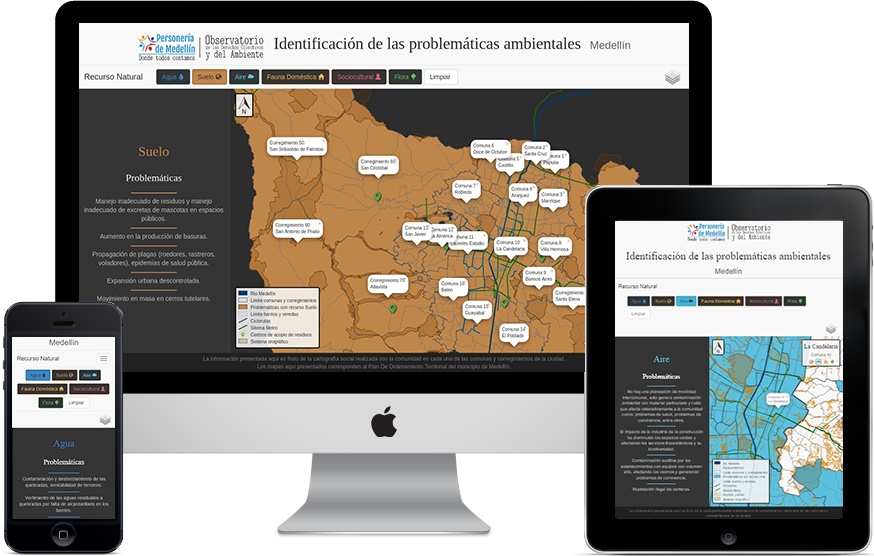
\includegraphics[width=0.7\textwidth]{../assets/images/responsive.png}
\caption{Demostración de diseño responsive. Esta imagen puede encontrarse en:\\ {\tt assets/images/responsive.png}}\label{fig:responsive}
\end{figure}

\section{Distribución y estructura del proyecto}


\begin{figure}[ht!]
\centering
\begin{subfigure}{.29\textwidth}
\begin{BVerbatim}
mdlln-map
├── app
├── assets
├── bower_components
├── bower.json
├── dist
├── doc
├── gulpfile.js
├── node_modules
├── package.json
├── README.md
└── test
\end{BVerbatim}
\caption{Raíz del proyecto.}\label{fig:root}
\end{subfigure}
\hfill
\begin{subfigure}{.29\textwidth}
\begin{BVerbatim}
app
├── favicon.ico
├── index.html
├── robots.txt
├── scripts
│   ├── comcorr.js
│   ├── leaflet-src.js
│   ├── main.js
│   └── resources.js
├── styles
│   ├── images
│   ├── leaflet.css
│   └── main.scss
├── support_maps
└── tutorial
\end{BVerbatim}
\caption{Código fuente del aplicativo.}\label{fig:app}
\end{subfigure}
\hfill
\begin{subfigure}{.29\textwidth}
\begin{BVerbatim}
dist
├── favicon.ico
├── fonts
├── index.html
├── robots.txt
├── scripts
│   ├── main.js
│   ├── plugins.js
│   └── vendor.js
├── styles
│   ├── images
│   ├── main.css
│   └── vendor.css
├── support_maps
└── tutorial
\end{BVerbatim}
\caption{Directorio de distribución.}\label{fig:dist}
\end{subfigure}
\caption{Estrucura de directorios del proyecto.}
\end{figure}

\subsection{Directorio raíz}
El directorio raíz del proyecto se muestra en la figura \ref{fig:root}. Los archivos fuente de la aplicación se encuentran en el directorio {\tt app}. La documentación, su fuente en \LaTeX\ y este documento pueden encontrarse en el directorio {\tt doc}. El directorio dist es generado automáticamente al compilar el proyecto y contiene los archivos necesarios para compartir la plataforma online u offline según la configuración. 

Los archivos: {\tt bower.json}, {\tt gulpfile.js} y {\tt package.json} corresponden a los archivos de configuración del entorno de desarrollo y los administradores de paquetes. Estos son los encargados de generar los directorios {\tt bower\_components}, {\tt dist}, {\tt node\_modules} y {\tt test}. Se recomienda prudencia al modificarlos, Los directorios {\tt bower\_components} y {\tt node\_modules} algunas dependencias fundamentales para la compilación del proyecto.

Finalmente el archivo {\tt README.md}, contiene una guía para configurar un entorno de desarrollo en formato markdown.

\subsection{Código fuente del aplicativo}

En el directorio {\tt app} se encuentran los archivos fuente del aplicativo. La estructura del directorio se puede apreciar en la figura \ref{fig:app}. Se destacan en este directorio los archivos {\tt index.html}, {\tt main.js} y {\tt main.scss}. El aplicativo reside fundamentalmente en estos tres archivos, donde el primero contiene la estructura del contenido, el segundo las funciones y declaraciones de Javascript necesarias para su interactividad y el tercero la información de los estilos para el contenido. Este ultimo en formato SASS \cite{sass} que posteriormente será compilado en un archivo CSS.

Los archivos {\tt leaflet-src.js} y {\tt leaflet.css} corresponden al framework para mapas interactivos Leaflet.

En el directorio {\tt support\_maps} se encuentra la información de los mapas en formato geoJson (Formato popular para contenido cartográfico en la web.). 

En el directorio {\tt tutorial} se encuentran las imágenes {\tt .gif} mostradas en el manual de usuario del aplicativo.

Los archivos dentro de la carpeta {\tt app/styles/images/} son necesarios para la correcta presentación de la información. Entre estos se encuentran los logos institucionales, etc.

\subsection{Activos del proyecto}

En la capeta {\tt assets} del directorio raíz pueden encontrarse los mapas originales usados para el proyecto en diferentes formatos ({\tt raw\_maps.zip}), así como imágenes e impresiones de pantalla del aplicativo final ({\tt assets/images/}). Cómo se mencionó antes, los mapas en formato geoJson pueden ser encontrados en {\tt app/support\_maps/} y las imágenes animadas mostradas en el manual de usuario en {\tt app/tutorial/}.

\begin{figure}[hb!]
\centering
\begin{subfigure}{.49\textwidth}
	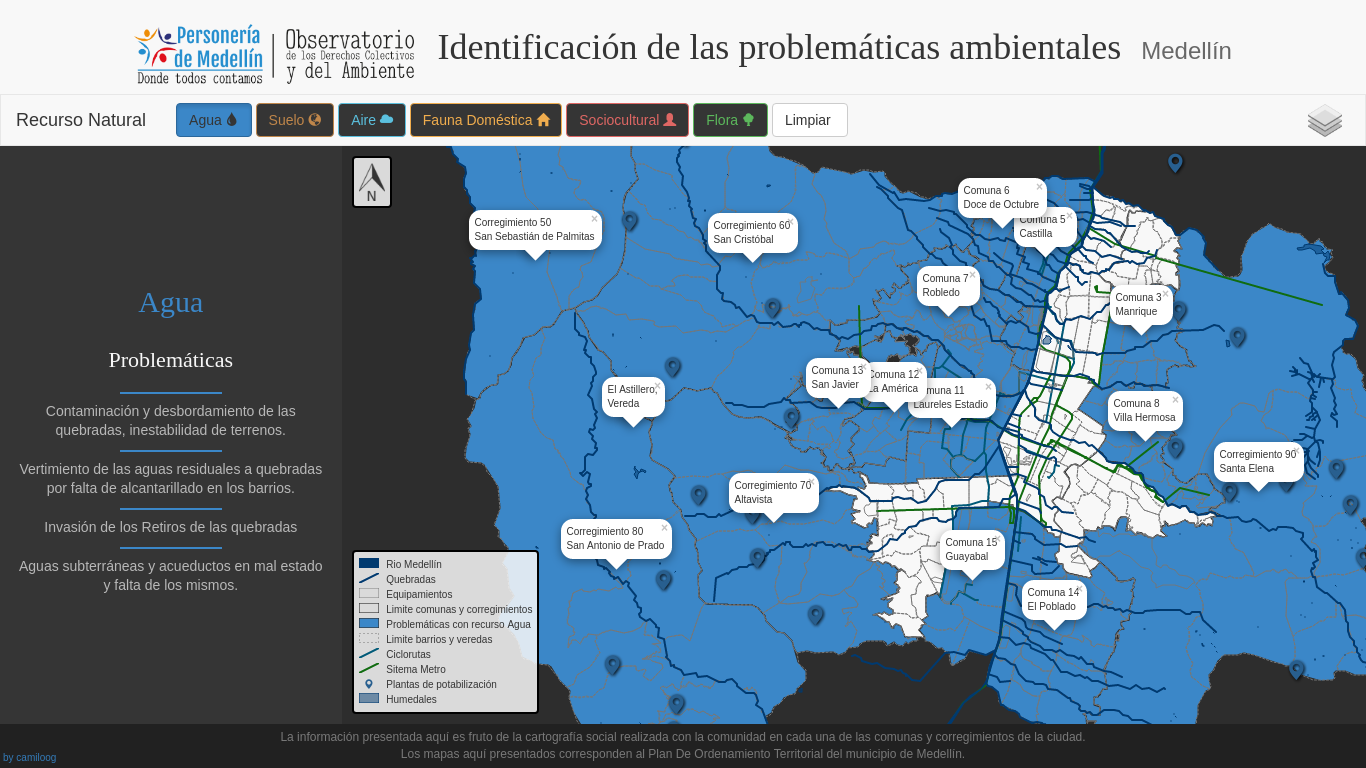
\includegraphics[width=\textwidth]{../assets/images/recurso_natural/recurso_agua.png}
	\caption{Agua}\label{fig:rAgua}
\end{subfigure}	
\hfill
\begin{subfigure}{.49\textwidth}
	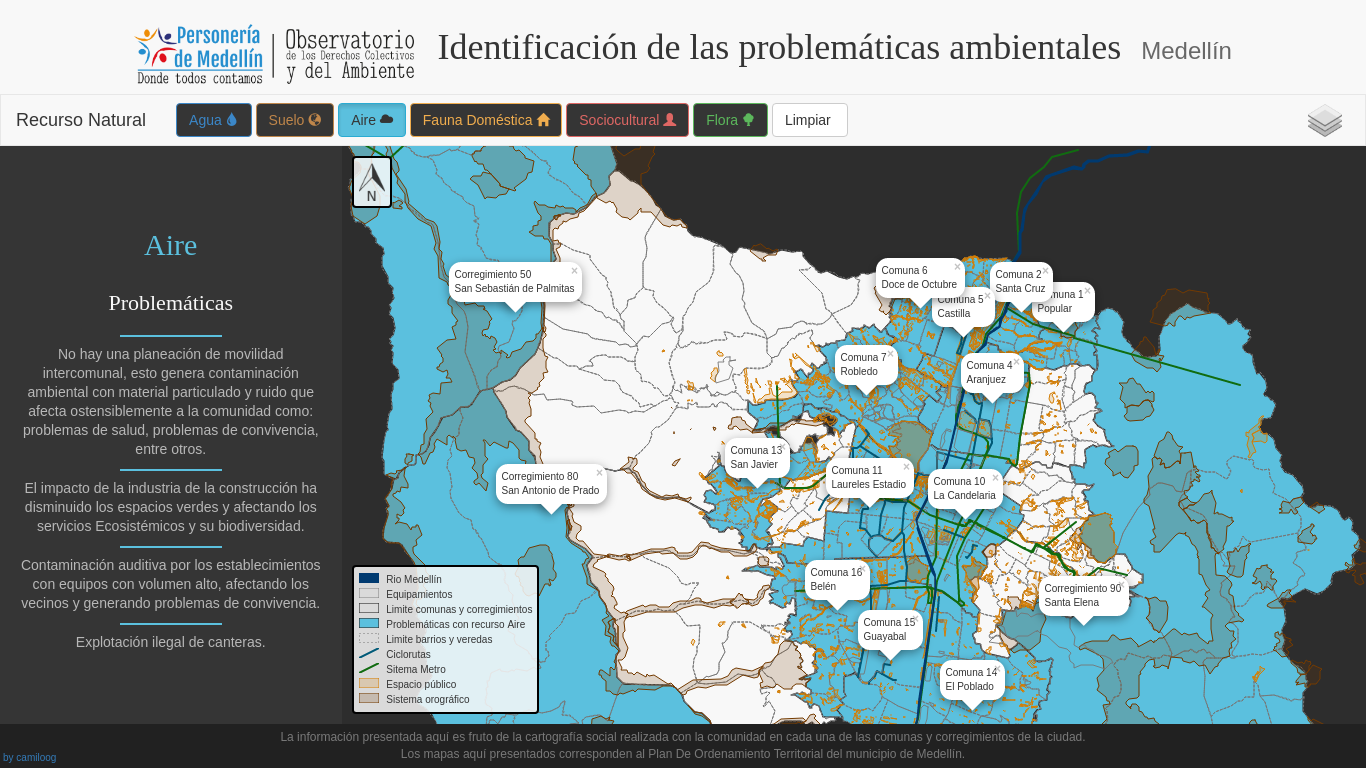
\includegraphics[width=\textwidth]{../assets/images/recurso_natural/recurso_aire.png}
	\caption{Aire}\label{fig:rAire}
\end{subfigure}

\begin{subfigure}{.49\textwidth}
	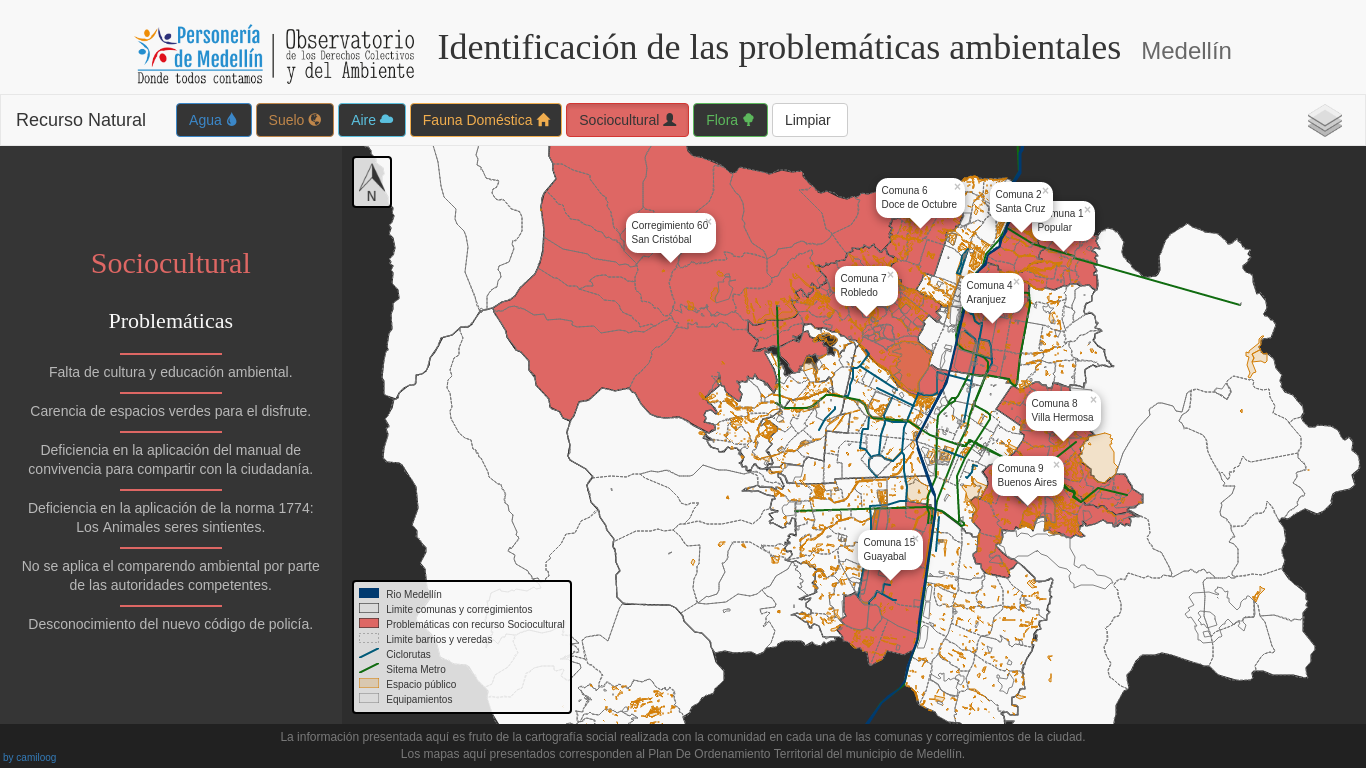
\includegraphics[width=\textwidth]{../assets/images/recurso_natural/recurso_sociocultural.png}
	\caption{Sociocultural}\label{fig:rSociocultural}
\end{subfigure}	
\hfill
\begin{subfigure}{.49\textwidth}
	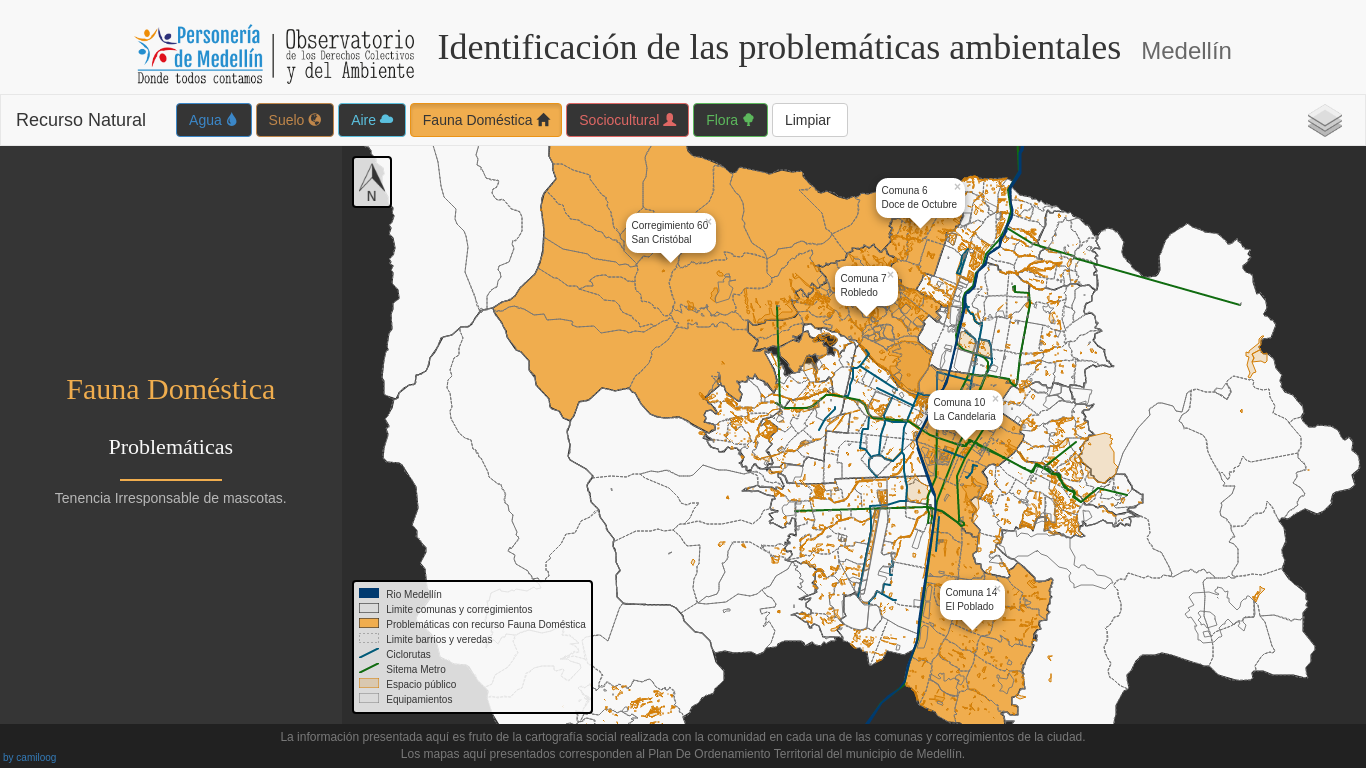
\includegraphics[width=\textwidth]{../assets/images/recurso_natural/recurso_fauna_domestica.png}
	\caption{Fauna doméstica}\label{fig:rFauna}
\end{subfigure}				

\begin{subfigure}{.49\textwidth}
	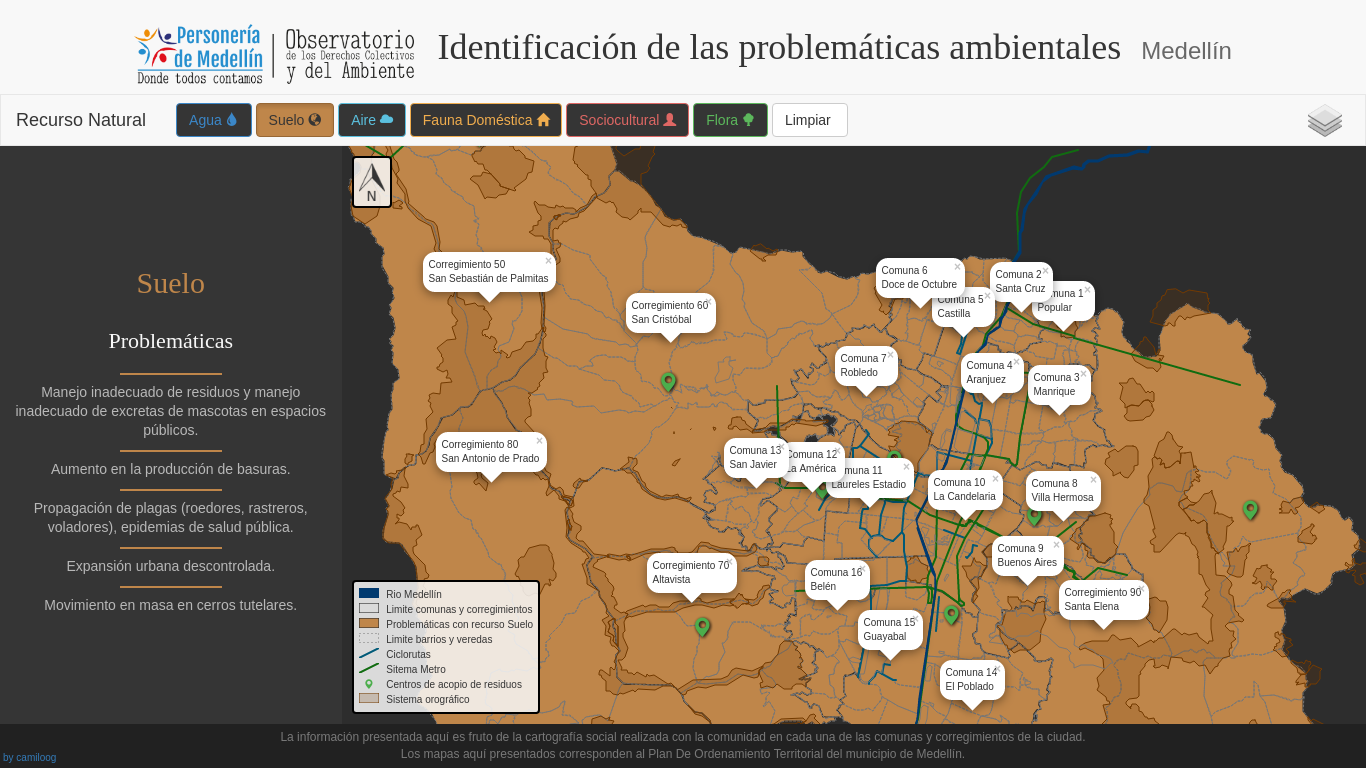
\includegraphics[width=\textwidth]{../assets/images/recurso_natural/recurso_suelo.png}
	\caption{Suelo}\label{fig:rSuelo}
\end{subfigure}	
\hfill
\begin{subfigure}{.49\textwidth}
	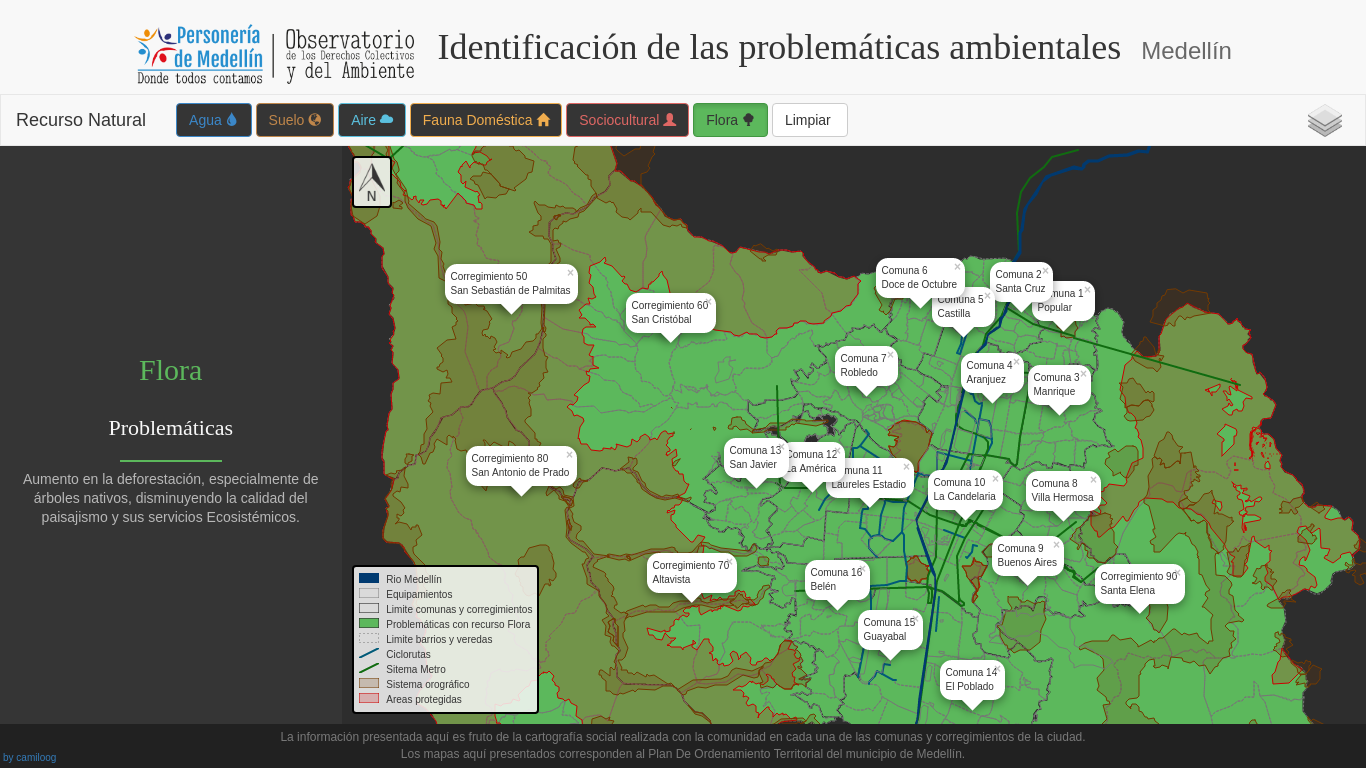
\includegraphics[width=\textwidth]{../assets/images/recurso_natural/recurso_flora.png}
	\caption{Flora}\label{fig:rFlora}
\end{subfigure}
\caption{Impresiónes de pantalla del aplicativo correspondentes a las problemáticas de cada recurso natural. Estas imágenes pueden ser encontradas en {\tt assets/images/recurso\_natural/}.}\label{fig:recurso}
\end{figure}

\subsection{Estructura del control de versiones}
El proyecto fue desarrollado haciendo uso del sistema de control de versiones Git. El proyecto cuenta con tres ramas: La rama {\tt master} donde se encuentra todo el desarrollo actualizado, compilado y optimizado para la web; la rama {\tt development} donde se realizan todos los desarrollos y pruebas antes de ponerlos en la rama {\tt master} y finalmente la rama {\tt offline-version} donde se optimiza la aplicación para su distribución {\it offline}.  

\subsection{Archivos para distribución}

La carpeta {\tt dist} contiene todos los archivos compilados y optimizados para su distribución, esta puede ser generada para publicar en la web desde las ramas {\tt development} y {\tt master} del control de versiones y optimizada para compartir {\it offline} desde la rama {\tt offline-version}. Sin embargo su estructura es similar en ambas compilaciones dado que al compilar los archivos fuente estos se minimizan y optimizan en la misma estructura. la estructura del directorio de distribución se muestra en la imagen \ref{fig:dist}. Los archivos {\tt vendor.css}, {\tt vendor.js} y {\tt plugins.js} corresponden a los {\it frameworks} y demás dependencias usadas.

\section{Configurar entorno de desarrollo para recompilar}

\subsection{Entorno de desarrollo}

Para contribuir en el desarrollo del proyecto o recompilarlo se recomienda un entorno Unix (Linux, Mac OS), pues facilita la ejecución del entorno desde una linea de comandos. 

Las siguientes dependencias deben ser instaladas en caso de no contar con ellas: {\tt node.js}, su administrador de paquetes {\tt npm} y {\tt gulp}.

Se debe copiar el contenido del CD con el proyecto completo en un directorio o clonar el repositorio mediante git desde \url{https://github.com/camiloog/mdlln-map}. Luego de hacerlo ingrese en el directorio del proyecto:
\begin{lstlisting}
	git clone https://github.com/camiloog/mdlln-map.git
	cd mdlln-map
\end{lstlisting}
Estando dentro del directorio del proyecto instalamos las dependencias necesarias:
\begin{lstlisting}
	npm install
  	bower install
\end{lstlisting}
Para montar y visualizar el proyecto en un servidor local (Configurado por las dependencias) simplemente ejecutamos la tarea {\tt serve} de la configuración de {\tt gulp}.
\begin{lstlisting}
	gulp serve
\end{lstlisting}
Para generar los archivos de distribución ejecutamos:
\begin{lstlisting}
	gulp serve:dist
\end{lstlisting}
Que generará la carpeta {\tt dist} y montará el resultado en un servidor local.

\subsection{Optimización web vs optimización offline}

Como se mencionó antes, el sistema de control de versiones cuenta con una rama optimizada para la web ({\tt development} o {\tt master}) y una rama optimizada para su visualización offline ({\tt offline-version}). En la versión web se cuenta con llamados al servidor a través de Ajax (Http request) para cargar los mapas requeridos de forma dinámica. Esto permite una mejor experiencia de usuario dado que los mapas no se descargan al tiempo, se descargan y grafícan según sean necesarios y el aplicativo se percibe más fluido. En la versión {\it offline} no se cuenta con un servidor que atienda a los los llamados de Ajax, por lo que todos los mapas deben ser cargados al iniciar el aplicativo. A pesar de que no hay que descargar ningún archivo porque se cuenta con todos de forma local la aplicación offline tarda unos segundos en cargar todas las variables Javascript necesarias en el navegador. La versión {\it offline} puede ser compartida en un CD y visualizada en cualquier navegador.

Para compilar la versión optimizada para la web ingrese en la rama {\tt development} dentro del directorio del proyecto y ejecute la tarea {\tt serve:dist}.
\begin{lstlisting}
	cd mdlln-map
  	git checkout development
  	gulp serv:dist
\end{lstlisting}
Para compilar la versión {\it offline}:
\begin{lstlisting}
	cd mdlln-map
  	git checkout offline-version
  	gulp serv:dist
\end{lstlisting}

\subsection{Consideraciones para modificar el código}
El aplicativo reside principalmente en los archivos {\tt app/scripts/main.js} y {\tt app/styles/main.scss}. El código Javascript fue diseñado para estar encapsulado en funciones auto invocadas que permiten un diseño modular. Se recomienda continuar con este paradigma y comentar apropiadamente las funciones y variables para un código mantenible.

\section{Manual de Usuario}
A parte de este manual técnico se hace entrega de un manual de usuario con soportes gráficos que permitan al usuario entender el funcionamiento y herramientas del aplicativo. Este manual puede encontrarse en el mensaje de bienvenida de la aplicación. Los soportes gráficos pueden ser encontrados en {\tt app/tutorial}.

\section{Características responsive}
La plataforma fue diseñada pensando en un aplicativo responsive bajo la filosofía {\it mobile first}. Esto implica que la distribución de los elementos en pantalla se auto ajustan y optimizan según el tamaño de la ventana o dispositivo tal como se muestra en la imagen \ref{fig:responsive}. 

\bibliographystyle{unsrt}
\bibliography{references}

\end{document}